\documentclass[12pt,onecolumn,a4paper]{article}
%landscape:横排
\usepackage{geometry}
\usepackage[utf8]{inputenc}
\usepackage{CJKutf8}
\usepackage{indentfirst}
\usepackage{setspace}
\usepackage{amsmath}
\usepackage{mathrsfs}
\usepackage{amsfonts}
\usepackage{graphicx} 
\usepackage{natbib}
\usepackage{caption}
\usepackage{subfigure}
\usepackage{subfig}
\usepackage{color}
\usepackage{booktabs}

%\usepackage{times}

\usepackage[justification=centering]{caption}%图片标题居中

%\usepackage{algorithm}  
%\usepackage{algorithmicx}  
%\usepackage{algpseudocode} 

\usepackage[vlined,ruled]{algorithm2e}
\usepackage{algorithmicx}
\usepackage[noend]{algpseudocode}

%\floatname{algorithm}{Algorithm} 
\renewcommand{\algorithmicrequire}{\textbf{输入:}}  
\renewcommand{\algorithmicensure}{\textbf{输出:}}

\newtheorem{definition}{定义}[section]
\newtheorem{proof}{Proof}
\newtheorem{lemma}{Lemma}[section]
\newtheorem{question}{Question}[section]
\newtheorem{Symbol}{Symbol}[section]
%\setlength{\parindent}{2em}
\geometry{left=2cm,right=2cm,top=2.5cm,bottom=2.5cm}
\def\cmt{\textcolor{blue}}
\def\todo{\textcolor{red}}
\def\cbl{\textcolor{blue}}
\newcommand{\DD}{\mathrm{\mathcal{D}}}
\newcommand{\HH}{\mathrm{\mathcal{H}}}
\newcommand{\aka}{\emph{a.k.a.}\xspace}

\title{\textbf{COMP 5711 - Advanced Algorithms} \ \textbf{Written Assignment \# 2}}
\author{ZHAO, Xi \\12256508 \\xzhaoca@connect.ust.hk}
%\date{Nov 2018}
\begin{document}
\maketitle

\section*{Amortized Analysis (CLRS Ch 17)}
\subsection*{Problem 17-2}
\subsubsection*{(a)} 
There are at most $k+1=O(\log n)$ sorted arrays and we requires search all of them in the worst case. The time of search in each array is bounded by $O(\log 2^i)\le O(\log n)$. So, the total query time becomes $O(k\log n)=O(\log^2 n)$.

\subsubsection*{(b)} 
As said in the problem, we build a sorted array of size $2^i$, whose elements are all those from the arrays of size $2^{i-1},\dots,2^0$, plus the new element. So, the insertion cost comes from merging these $i$ sorted arrays. The cost of merging two sorted arrays of size $l_1$ and $l_2$ is $l_1+l_2$. So, the cost of merging these $i$ sorted arrays is 
$$\sum_{j=0}^{i-1} 2^j=2^i-1.$$ The cost of inserting an new element into these array is also $O(2^i)$. Therefore, the total cost is $O(2^i)$.

\subsubsection*{(c)} 
Let $i^*=\min\{i|b_i=0,n=\overline{b_kb_{k-1}\cdots b_0}\}$. When insert a new element, we will merge all arrays of size $2^{i^*-1},\dots,2^0$ when $i^*>0$, which is $O(2^{i^*})$. Is is obvious that
$$\Pr[i^*=0]=\Pr[b_0=0]=1/2,$$
$$\Pr[i^*=1]=\Pr[b_0\neq0,b_1=0]=1/2^2,$$
$$...$$
$$\Pr[i^*=j]=\Pr[b_k\neq0,0\le k<j]\cdot\Pr[b_j=0]=1/2^{j+1}.$$
The amortized cost of an insertion is
$$T=\sum_{j=0}^{k} \Pr[i^*=j]O(2^j)=\sum_{j=0}^{k} \frac{1}{2^{j+1}}O(2^j)=\sum_{j=0}^{k} O(1)=O(k)=O(\log n).$$
\subsection*{Problem 17-3}
\subsubsection*{(a)} 
To rebuild the subtree with size $n_i$, we write down all elements in this subtree orderly by using an inorder traversal in this subtree, which costs $O(n_i)$ time. Then, we build a binary tree on these elements as balanced as possible. Specifically, we select the median of the list to be the root, and recurse on the two halves of the list that remain on both sides, which also costs $O(n_i)$ time. The rebuilt subtree is $1/2$-balanced and inherently $\alpha$-balanced for $1/2<\alpha<1$. The total time used is $O(n_i)+O(n_i)=O(n_i)$.
\subsubsection*{(b)}
First, we prove the height $h$ of an $\alpha$-balanced binary tree with size $n$ is at most $O(\log n)$.
For an $\alpha$-balanced binary tree with size $n$. The size of the node in the layer $0$ (the top layer) has the size $n$; the size of the nodes in the layer $1$ have the size at most $\alpha\cdot n$ by the definition. Recursively, it is obvious that the size of the nodes in the layer $l$ have the size at most $\alpha^l\cdot n$. Let $h$ be the height of this tree, we have $\alpha^h\cdot n\le 1$, indicating that $h\le \log_\alpha n=O(\log n).$ For an insertion or deletion as in an ordinary binary tree, its cost is $O(h)=O(\log n)$

Then, we consider the amortized cost for rebuilding a subtree. For a node $e_i$ with the size $n_i$ that is just rebuilt, it will be $1/2$-balanced. 
Assume after $x$ insertions or deletions, $e_i$ becomes out of balance and requires to be rebuilt. Hence, for each insertion or deletion, the amortized cost is $O(n_i/x)$. So, what is the minimum of $x$? In the worst case for insertion, all $x$ elements are all inserted into the left subtree of $e_i$ or the right subtree of $e_i$. In this case, $1/2 n_i+x>\alpha (n_i+x)$, having $x>\frac{\alpha-1/2}{1-\alpha} n_i=O(n_i)$. Similarly, we can prove the minimal $x$ for deletion is also $O(n_i)$. The amortized cost for each insertion or deletion on node $e_i$ can be $O(n_i/x)=O(1)$. Next, we can find that each insertion or deletion only incurs at most one node to be rebuilt per layer. So, each insertion or deletion have a $O(h)$ amortized cost on all binary tree.

Therefore, the total amortized cost of each insertion/deletion is $O(\log n)$.

\subsection*{Problem A}
%\begin{figure}[]
%	\centering
%	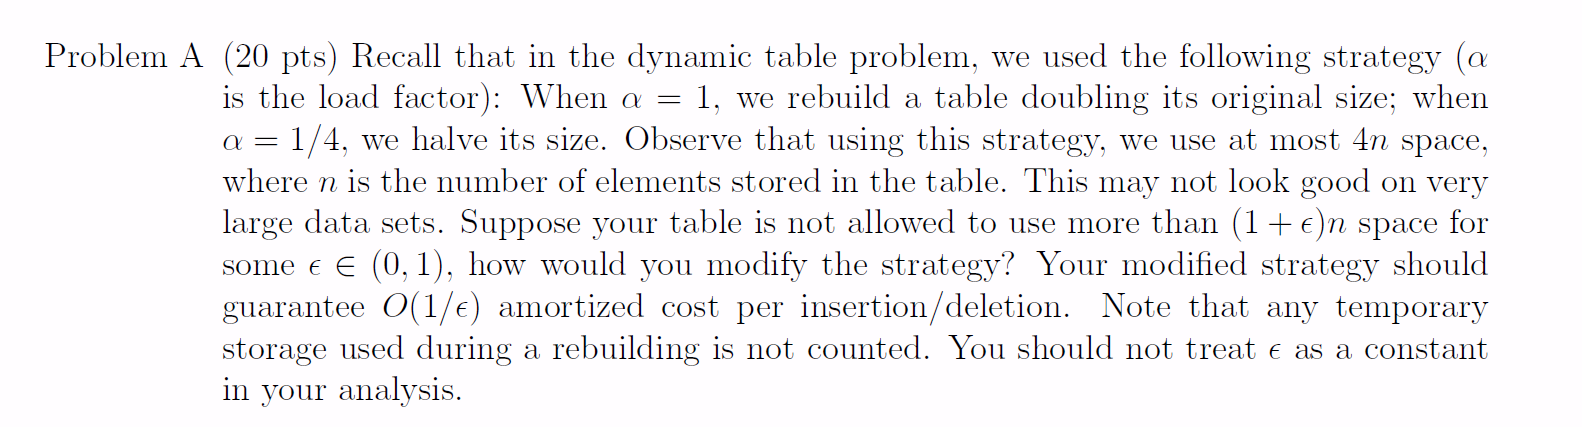
\includegraphics[width=0.95\textwidth]{prob3.png}
%	\caption{Problem A} 
%	\label{fig:prob3}
%\end{figure}
Let $\alpha_0=1/\sqrt{1+\epsilon}$, we modify our strategy as: when $\alpha=1$, we rebuild a table with $1/\alpha_0$ times as larger as its original size; when $\alpha=\alpha_0^2$, we reduce its size $\alpha_0$ times as smaller as its size. In this case, we always have $\alpha>\alpha_0^2=\frac{1}{1+\epsilon}$ and no more than $(1+\epsilon)n$ space is used. As that in an original dynamic table, the potential function of this dynamic table is
\begin{equation}
	\Phi(T)=
	\begin{cases}
		\frac{1}{1-\alpha_0}\cdot(T.num-\alpha_0 T.size)&, \alpha(T)\ge \alpha_0\\
		\frac{\alpha_0}{1-\alpha_0}\cdot(\alpha_0 T.size-T.num)&, \alpha(T)< \alpha_0
	\end{cases}
\end{equation}
%$$\Phi(T)=\frac{1}{1-\alpha_0}\cdot|T.num-\alpha_0 T.size|.$$
When $T.num=\alpha T.size$, $\Phi(T)=0$ as desired; when $T.num=T.size$ or $T.num=\alpha_0^2T.size$, we have $\Phi(T)=T.num$ as desired. 

Then, we analyze the amortized cost of this strategy. Denote $n_i$ and $s_i$ as the $T.num$ and $T.size$ after $i$th operation.
We start with the case in which the $i$th operation is TABLE-INSERT. 
%When $\alpha_{i-1}\ge $
\begin{itemize}
	\item [\textbf{Case I1}]: \textbf{(No expansion is triggered.)} In this case $n_i=n_{i-1}+1$ and $s_i=s_{i-1}$
	\begin{equation*}
		\begin{split}
			\hat{c_i}=&c_i+\Phi_i-\Phi_{i-1}\\
			%=&1+\frac{1}{1-\alpha_0}|n_i-\alpha_0s_i|-\frac{1}{1-\alpha_0}|n_i-1-\alpha_0s_i|\\
			\le&1+\frac{1}{1-\alpha_0}|(|n_i-\alpha_0s_i|-|n_i-1-\alpha_0s_i|)|\\
			\le&1+\frac{1}{1-\alpha_0}
		\end{split}
	\end{equation*}
	\item [\textbf{Case I2}]: \textbf{(An expansion is triggered.)} In this case we have $n_{i-1}=s_{i-1}$, $n_i=n_{i-1}+1$ and $s_i=\frac{1}{\alpha_0}s_{i-1}$. Also, in this case, we have $\alpha(T)\ge \alpha_0$. Hence,
	\begin{equation*}
		\begin{split}
			\hat{c_i}=&c_i+\Phi_i-\Phi_{i-1}\\
			=&n_i+\frac{1}{1-\alpha_0}|n_i-\alpha_0\cdot \frac{1}{\alpha_0}(n_i-1)|-\frac{1}{1-\alpha_0}|n_i-1-\alpha_0(n_i-1)|\\
			=&n_i+\frac{1}{1-\alpha_0}-(n_i-1)\\
			=&1+\frac{1}{1-\alpha_0}
		\end{split}
	\end{equation*}
\end{itemize}

We next consider the case in which the $i$th operation is TABLE-DELETE. 
%When $\alpha_{i-1}\ge $
\begin{itemize}
	\item [\textbf{Case D1}]: \textbf{(No contraction is triggered.)} In this case $n_i=n_{i-1}-1$ and $s_i=s_{i-1}$
	\begin{equation*}
		\begin{split}
			\hat{c_i}=&c_i+\Phi_i-\Phi_{i-1}\\
			%=&1+\frac{1}{1-\alpha_0}|n_i-\alpha_0s_i|-\frac{1}{1-\alpha_0}|n_i+1-\alpha_0s_i|\\
			\le&1+\frac{1}{1-\alpha_0}|(|n_i-\alpha_0s_i|-|n_i+1-\alpha_0s_i|)|\\
			\le&1+\frac{1}{1-\alpha_0}
		\end{split}
	\end{equation*}
	\item [\textbf{Case I2}]: \textbf{(A contraction is triggered.)} In this case we have $n_{i-1}=\alpha_0^2 s_{i-1}$, $n_i=n_{i-1}-1$ and $s_i={\alpha_0}s_{i-1}$. Also, in this case, we have $\alpha(T)< \alpha_0$. Hence
	\begin{equation*}
		\begin{split}
			\hat{c_i}=&c_i+\Phi_i-\Phi_{i-1}\\
			=&n_i+1+\frac{\alpha_0}{1-\alpha_0}|n_i-\alpha_0\cdot \frac{1}{\alpha_0}(n_i+1)|-\frac{\alpha_0}{1-\alpha_0}|n_i+1-\alpha_0\cdot\frac{1}{\alpha_0^2}(n_i+1)|\\
			=&n_i+1+\frac{\alpha_0}{1-\alpha_0}-(n_i+1)\\
			=&\frac{\alpha_0}{1-\alpha_0}
		\end{split}
	\end{equation*}
\end{itemize}

Therefore, in any of these four cases, the amortized cost is bounded by 
$$1+\frac{1}{1-\alpha_0}=1+\frac{1}{1-1/\sqrt{1+\epsilon}}=1+\frac{\sqrt{1+\epsilon}}{\sqrt{1+\epsilon}-1}<1+\frac{2}{\epsilon/4}=O(1/\epsilon).$$
\section*{Randomized Algorithms (KT Ch 13)}
\subsection*{Problem 1}
Our algorithm is coloring every node in the graph independently by using one of the three colors with probability $1/3$, which can be done in $O(m)$ time. In this case, the probability that an edge $e=(u,v)$ is satisfied is 
$$\Pr[u.color\neq v.color]=1-1/3=2/3.$$
Since the probability that the edge is satisfied are independent to each other, the number of expected satisfied edges are $\frac{2}{3} m\ge \frac{2}{3} c^*.$
\subsection*{Problem 7}
\subsubsection*{(a)} 
For a clause $C_i$ with $n_i$ variables, the probability that it is satisfied is $1-1/2^{n_i}\ge1/2$. So, the expected number of clauses satisfied is at least $1/2\dot k=k/2.$

Consider instances $\{x_1,\bar{x_1},x_2,\bar{x_2},\cdots,x_n,\bar{x_n}\}.$ No matter how we assign the variable, only one of two conflicting clauses can be satisfied. Therefore, no assignment satisfies more than
$k/2$ clauses.
\subsubsection*{(b)} 
Consider there are totally $k$ clauses where $k_1$ of them are single-variable and $k_2=k-k_1$ of them are multi-variable. We design our algorithm for different two cases:
\begin{itemize}
	\item [\textbf{Case 1}]: When $k_1\ge0.6 k$, we assign the variables to make all single-variable clause satisfied. Since there are no conflict clauses, it is doable. So, the number of satisfied clauses is at least $k_1\ge 0.6k$.
	\item [\textbf{Case 2}]: When $k_1<0.6 k$, we assign each variable independently to true or false with probability $1/2$. In this case, the multi-variable clause is satisfied with at least probability $1-1/4=0.75$ and the single-variable clause is satisfied with probability $0.5$.
	The expected number of satisfied clauses is 
	$$N>0.75(k-k_1)+0.5k_1=0.75k-0.25k_1>0.75k-0.25\times 0.6k=0.6k.$$
\end{itemize}
In either case, the expected number of satisfied clauses is at least $0.6k.$
\subsubsection*{(c)} 
Assume there are $2m$ conflicting clauses, \textsf{OPT} is hence less then $k-m$. We remove these $2m$ conflicting clauses and adopt the algorithm described in (b) on the remaining $k-2m$ clauses. The expected number of satisfied clauses is at least $0.6(k-2m)+m\ge 0.6(k-m)=0.6\cdot\empty$\textsf{OPT}.


\end{document}

